\documentclass{sig-alternate}
\usepackage{amsmath}
\usepackage{amssymb}
\usepackage{proof}
\usepackage{url}
\usepackage{color}

\newcommand{\todonote}[1]{\textcolor{blue}{{\bf TODO:} {\it #1}}}
\newcommand{\comment}[1]{\textcolor{red}{{\bf COMMENT:} {\it #1}}}

\newcommand{\arr}[1]{\ensuremath\xrightarrow{#1}}

\begin{document}

\title{A Type-based Approach to Separating\\Protocol from Application Logic:\\A Case Study in Hybrid Computer Programming}

\numberofauthors{3}

\author{
% 1st. author
\alignauthor Geoffrey C. Hulette\\
  \affaddr{University of Oregon}\\
  \affaddr{Eugene, OR}\\
  \email{ghulette@cs.uoregon.edu}
% 2nd. author
\alignauthor Matthew J. Sottile\\
  \affaddr{Galois, Inc.}\\
  \affaddr{Portland, OR}\\
  \email{mjsottile@computer.org}
% 3rd author
\alignauthor Allen D. Malony\\
  \affaddr{University of Oregon}\\
  \affaddr{Eugene, OR}\\
  \email{malony@cs.uoregon.edu}
}

\CopyrightYear{2012}

\maketitle

%!TEX root = twig-language.tex

\begin{abstract}

Twig's approach to typemapping, language design, and comparison to Swig.

\end{abstract}

%!TEX root = twig-language.tex

\section{Introduction}

Twig is a new language for writing \emph{typemaps} -- programs that transform data from one type to another, while preserving (as much as possible) the underlying value of the data. Typemaps have proven useful in many kinds of programming and especially automated code generation, where we require a transformation to pass a single nominal value across a pair of mismatched types that we know to be interchangeable in some way. The best-known example of this problem is found in multi-language programming. For example, a programmer may wish to pass a Python integer to a C function, where a C int is expected. If we have a typemap that performs the transformation from Python integers to C integers, then an automated tool can generate the conversion code automatically, and expose the C function in Python via a generated wrapper.

There are a number of existing tools and languages for creating typemaps and generating code from them. Twig builds on existing typemap tools in several ways.

First, Twig's typemaps are composable, i.e., new typemaps may be constructed by combining old ones. Thus, complex typemap transformations may be built from simpler ones. Our notion of typemap composition is based on the formalisms used in Fig\cite{fig} and System S\cite{system-s}, but we extend and refine that work in some key ways.

Second, Twig incorporates a robust, formal model of code generation. This allows Twig to generate code based on typemaps in many different target languages.

Finally, Twig includes a facility for \emph{reducing} typemaps by exploiting identity relationships among typemap expressions. Some reductions are based on a universal ``algebra of typemaps,'' while others are domain-specific and must be described by the user. We have shown in prior work that typemap reduction can be used to optimize certain transformations. Reductions are covered in our previous work, and we will not address them further here.

In this paper, we will describe Twig's formal language structure, and then show how this structure allows us to express complex typemaps more concisely than with traditional tools. First, we review existing approaches to typemaps and related problems. Second, we present the semantics for Twig's code generation model, and then the semantics for the typemap language itself. Third, we present a typemap example in Swig, and show how the same problem can be solved more concisely and clearly in Twig. Finally, we conclude with ideas for future work.

%!TEX root = twig-gpu.tex

\section{Related Work}

Numerous systems have been created in recent years to address the GPU
programming problem that provide an abstraction above low level interfaces such
as OpenCL or CUDA. These include the PGI Accelerate model~\cite{pgi-accelerate}
or the HMPP programming system~\cite{hmpp}. While both of these systems provide
an abstraction above the low level programming library, we believe that they
hide too much from the programmer. There is little room for tuning of the way
the lower level interface to the accelerator is used -- the programmer is
reliant on the tool vendor to provide a sufficiently tunable abstraction such
that working with this low level interface is unnecessary.

Unfortunately, in large applications, it is infeasible to assume that all
developers of the components that form the overall application will use the same
higher level abstraction method. This makes it challenging not only to tune the
code that bridges between devices, but to reason about how the code resulting
from the independent programming systems interacts. We address this by adopting
a code generation approach in which a single, low level target is used (such as
OpenCL). This approach addresses both the composability problem (all Twig code
maps to a single ``lingua franca'' for programming the hybrid system), and
exposes the implementation in the generated code to allow tuning and
modification by the end user.

The closest work to that which we describe is Reppy's Application Specific
Foreign Function Interface Generator, FIG~\cite{reppy06fig}. In that work, a
similar formal approach was taken specifically to the generate bindings between
programs in two different programming languages. We have found that very similar
issues arise in building bindings between devices in a hybrid system. These
overlaps include memory ownership and management, data marshalling, and managing
the flow of program control across the language or device boundary. Our work
builds upon that of Reppy and Song, and aims to provide a general-purpose tool
that is not tied to the Moby programming language. Twig's approach largely
subsumes the case of foreign function interface generation, and could
incorporate other interesting applications like mapping between two different
libraries written in the same language. This second case is of particular
interest when dealing with the problem of composing complex software from
smaller program units, where developers working independently may have chosen
different representations for data types that are semantically identical.

Kennedy's \emph{telescoping languages} work is related to ours in that it seeks
to support high-level programming by deferring challenging problems to automated
tools. In particular, the telescoping languages effort sought to provide the
ability to build high-level problem-solving languages that used scripting
languages to coordinate functionality present in domain-specific
libraries~\cite{kennedy00telescoping}. Much of the work then focused on compiler
optimization methods and targeting potentially distributed, grid-based
environments. Interestingly, one of the compilation techniques that was called
out as part of the telescoping languages strategy was that of automated
recognition and exploitation of identities. This would allow a compilation tool
to recognize instances when compositions of functions could be replaced with
more efficient equivalent implementations. As is described in this paper, we
adopt a similar strategy in identifying compositions of rules that are
equivalent to the identity function and can therefore be eliminated.

Code generation approaches have had notable success in the computational science
field, an exemplar being the Tensor Contraction Engine
(TCE)~\cite{baumgartner05synthesis}. The TCE allows computational chemists to
write tensor contraction operations in a high level language similar to
Mathematica, leaving it up to the TCE tool to generate the corresponding
collections of loops that implement the operations. The advantage of this
approach is that tedious and often error-prone nested loops over many large
arrays with a correspondingly large number of indices can be both machine
generated and optimized. Optimizations such as loop fusion, memory locality
management, and data distribution and partitioning in a parallel machine can all
be automated, versus previous approaches that required very labor intensive hand
written code. The TCE is not a general tool, and is only of use to programmers
working with similar tensor-based computations.

%!TEX root = twig-gpu.tex

\section{Method Overview}

Our approach uses Twig to represent the protocol logic of a GPU-based program with extended type information. Twig's high-level structure allows for a clean mix of computational and protocol logic. In addition, we can track and constrain operations in the protocol logic using extended type information. In particular, we can use \emph{located types}, described in Section~\ref{sec:located-types}, to keep track of data as it moves between the CPU and GPU.

Protocol related logic is often concerned with allocation, movement, and representational conversion. Adding the concept of location to types supports a number of protocol operations, including automatic generation of allocation logic (corresponding to typed variable declaration and scoping), and device-specific representation marshalling. By extending the type system, we offload the burden of writing and optimizing this protocol logic from the programmer to automatic tools.

The advantage of pushing location information into the type system is that it forces programmers to explicitly account for operations related to the protocol logic of an application. In plain CUDA or OpenCL codes, protocol-related operations are intermixed with computational logic, and the type system does not help to enforce protocol rules. In CUDA, for example, the type system will not prevent a faulty program from executing a kernel on the GPU before the appropriate data has been copied. We will show that by augmenting type information, we can make many of these protocol-related details explicit and check them at compile time.

As we will see in Section~\ref{semantics}, programs written in Twig's language are constrained with respect to control flow. This is by design. Twig's simple semantics make its programs easy to reason about, and thus to transform via automated methods. In Section~\ref{sec:example} we will demonstrate one way in which we can exploit this property, by transforming GPU-related programs to eliminate redundant memory copies. 

Twig does not currently feature any built-in looping constructs. We are working to address this limitation -- see Section~\ref{sec:future-work}.

We illustrate the redundant memory copy problem in Fig.~\ref{basic-idea}. In the diagram, two GPU kernel transformations, $f$ and $g$, are called in sequence. The na\"ive composition is shown in Fig.~\ref{basic-idea}(a). This case has redundant data movement. The arrangement in Fig.~\ref{basic-idea}(b) is the desired composition, with the redundant intermediate copying operations eliminated.

\begin{figure}[ht]
\centering
\begin{tabular}{cc}
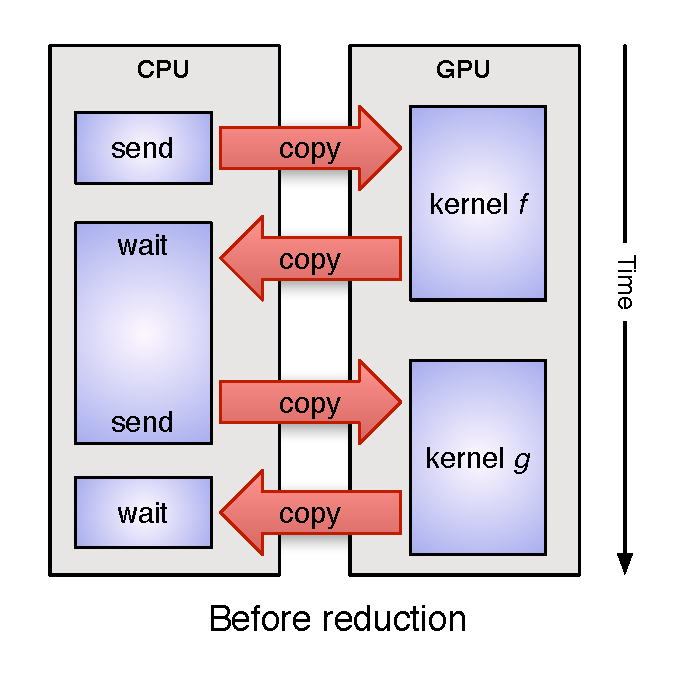
\includegraphics[width=2in]{images/reduction-before}&
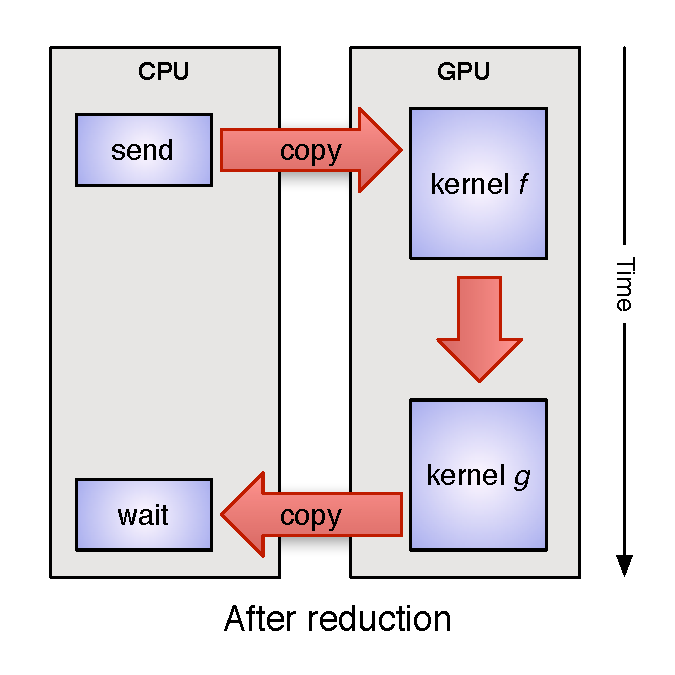
\includegraphics[width=2in]{images/reduction-after}\\
(a)&(b)\\
\end{tabular}
\caption{Elimination of redundant data movement. Part (a) depicts two GPU kernels called in sequence, unnecessarily copying data to and from the device. Part (b) shows the same program with the redundant copies removed.}
\label{basic-idea}
\end{figure}

Twig operates on data types instead of data. The input to a Twig program is a data type, and the output is a transformed data type along with some generated code that will perform the transformation on data in the target language. For this reason, Twig is restricted to operate only on types that can be represented in the target language, (e.g., for C, things like \texttt{int}, \texttt{float}, or \texttt{structs}). It can, however, augment the information about those types in order to make them more restrictive. For GPU programming, we exploit this capability with the addition of \emph{located types}.

Located types are a specific instance of the notion of \emph{augmented types}, in which the types provided by a base language are enhanced to carry important semantics that are implicit in the underlying language. For example, most languages support multi-dimensional arrays, but the ordering (column versus row major) is implicit. An augmented multi-dimensional array type would add this ordering as an explicit part of the type. In this way, the transition between representations would be explicit and clear in the code, instead of something implied by the base language itself.

\subsection{Located Types}
\label{sec:located-types}

For GPU programming, we augment standard data types with a  \emph{location}. The location information describes where the data is stored in memory, i.e., either in system memory or on the GPU.

For example, we can represent an array of \texttt{int}s on the CPU with the Twig type \texttt{array(int)}. The same type located on the GPU is \texttt{gpu(array(int))}. Any standard type may be wrapped inside the \texttt{gpu} type constructor.

Note that this location information is only used within Twig itself. In particular, it may or may not be reflected in the generated target type. If we are generating CUDA code, for example, the generated type for both \texttt{gpu(array(int))} and \texttt{array(int)} is simply a C pointer to \texttt{int} (i.e., \texttt{int *}). In this case, the location information is erased during the code generation phase. For other target languages or APIs that have a notion of location, the information could be preserved in the generated data types.

By augmenting basic data types with location information, we ensure that rules must be specific to the GPU in order to operate on GPU data. For example, a rule

\begin{verbatim}
[gpu(array(float)) -> gpu(array(int))]
\end{verbatim}

converts an ``array of floats'' data type to an ``array of integers'' type if and only if the type describes data located on the GPU. If the type describes data located elsewhere, its type must be ``converted'' (i.e., the data copied to the device) with a rule such as

\begin{verbatim}
[array(float) -> gpu(array(float))]
\end{verbatim}

This simple scheme enables automated reasoning about data motion.

It is important to understand that rules such as those given above describe transformations on \emph{data types}, not on the data themselves. It falls to the code that is generated as a consequence of successful application of these rules to perform the promised conversion on the actual data; this is described in Section~\ref{sec:code-gen}.

Located types could be used in more complex situations, as well. For example, they could be used track data moving between multiple GPU devices, with each device corresponding to a unique located type.

%!TEX root = twig-gpu.tex

\section{Code generation}
\label{sec:code-gen}

To generate code, Twig relies on an abstract, language-independent model with a small number of basic operations. This simplified model is useful for formulating Twig's semantics, described in Section~\ref{semantics}. It is also helpful in clarifying the precise operations which Twig supports, without getting bogged down in the (typically quite complicated) details of outputting code for a particular programming language.

Twig generates code in units called \emph{blocks}. The term ``block'' is somewhat overloaded -- our usage differs somewhat from the norm. In Twig, a block of code represents anything that performs some operation on a set of inputs, and which produces a set of outputs. Blocks may have zero or more inputs and outputs. Blocks can also be combined in two different ways: \emph{sequentially}, or \emph{in parallel}. These operations are described in more detail below.

Our current implementation of this model supports the generation of C code, and adds some extra features to support that language. These features include such details as managing type declarations, support for parameterized blocks, and for ``closing'' blocks, which are generated as variables go out of scope and are intended to be used to free resources. We are looking into the possibility of incorporating these and other features into the language-neutral model, but for the moment they are specific to C.

\begin{figure}[ht]
\centering
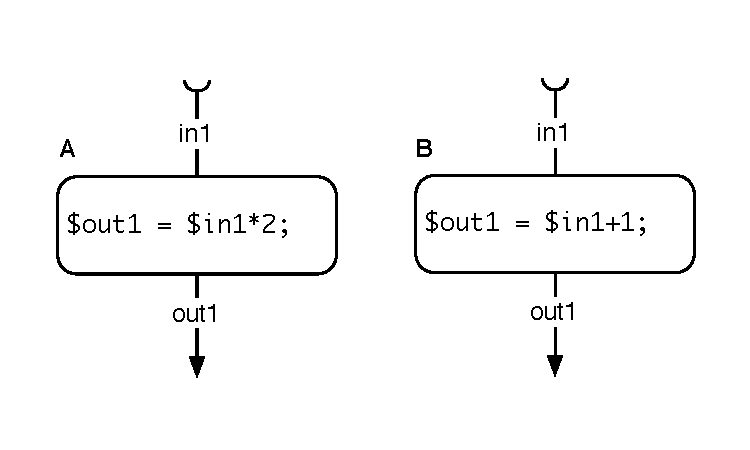
\includegraphics[width=\columnwidth]{images/code-gen1}
\caption{Two basic blocks, A and B.}
\label{fig:codegen-blocks}
\end{figure}

\subsection{Block Composition}

As mentioned above, Twig provides two fundamental binary operations on blocks. The first is the \emph{sequential composition} operator, represented by the addition symbol ($+$). Sequencing connects two blocks of code by ``wiring'' the outputs of the first block into the inputs of the second. In C, this is done by creating temporary variables which are substituted into the original blocks. For example, see Figure~\ref{fig:codegen-seq}, which builds on Figure~\ref{fig:codegen-blocks}.

\begin{figure}[ht]
\centering
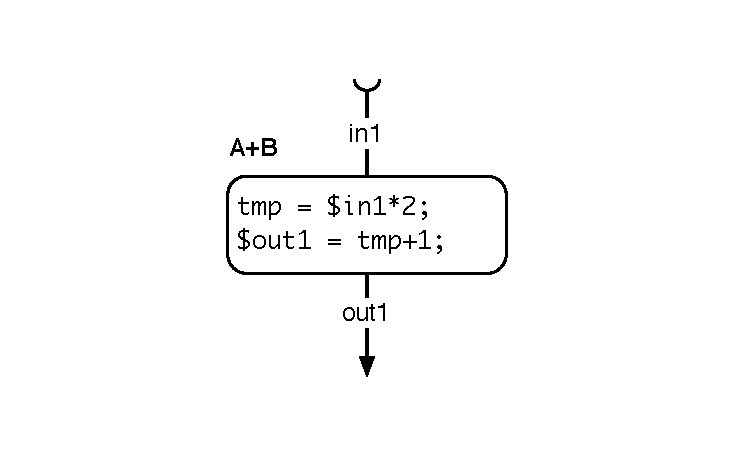
\includegraphics[width=\columnwidth]{images/code-gen2}
\caption{Two blocks from Figure~\ref{fig:codegen-blocks} composed sequentially. The variable ``tmp'' is created, and renaming performed, so that the output of block A would flow to the input of block B.}
\label{fig:codegen-seq}
\end{figure}

Twig's implementation takes care of declaring and uniquely naming temporary variables to accomplish sequencing.

The second operator is \emph{parallel composition}. Under this operator, two blocks are combined so as to execute independently of one another, but to appear as one single block. We represent this operation with the multiplication operator ($\times$). An example is shown in Figure~\ref{fig:codegen-par}.

\begin{figure}[ht]
\centering
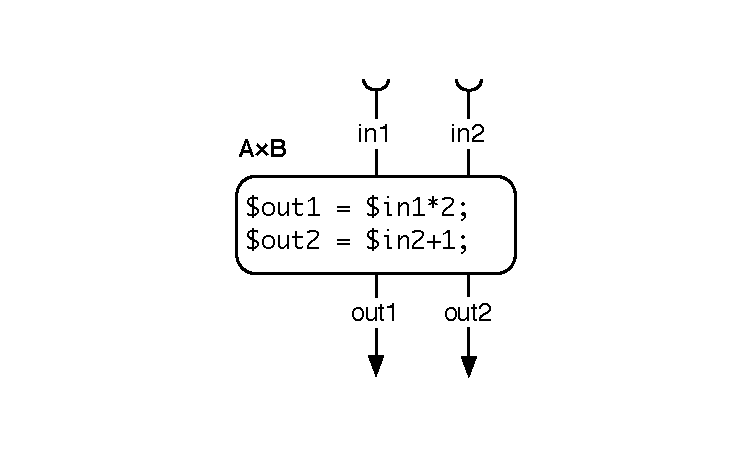
\includegraphics[width=\columnwidth]{images/code-gen3}
\caption{Two blocks from Figure~\ref{fig:codegen-blocks} composed in parallel. Renaming is performed such that the composed block has two inputs and two outputs.}
\label{fig:codegen-par}
\end{figure}

\subsection{Special Blocks}

Twig defines a special set of blocks called \emph{permutation} blocks. These blocks have some special properties, which we will exploit for the purposes of rewriting programs to remove redundant memory copies. In particular, some kinds of blocks act as a kind of identity element when composed with others.

The permutation blocks are referred to as $\Pi_m(i_1,\ldots,i_n)$, and represent the primitive operation of rearranging $m$ inputs to $n$ outputs, possibly in a different order, and possibly duplicating or dropping elements. The data is only passed through, and are otherwise unchanged.

Among the permutation blocks, there are a set of elements for which we provide special rules; namely, a set of \emph{identity} permutations. The simplest of these is $\Pi_1(1)$, which acts as an identity transformation with one input and one output. We refer to this element as $I_1$. In fact, there are an unlimited number of identity transformations, which take $n$ inputs to $n$ outputs, unchanged. These are referred to as $I_n$, where $1 \leq n$, and $I_n = \Pi_n(1,2,\ldots,n)$. The blocks $I_n$ are left- and right-identity elements under a sequence operation. We sometimes use $I_n$ as a kind of ``no-op.''

Using this simple system, a wide variety of code can be generated.

%!TEX root = twig-gpu.tex

\section{Twig's Semantics}
\label{semantics}

Twig is based on a core semantics called System S~\cite{Visser:1998p333},
augmented with semantics for generating code and specialized to operate on types
instead of general terms. Twig uses the operators of System S to combine
primitive \emph{rules} into more complex transformations on types. These
transformations are then applied to a given type, resulting in a new type and
generating code as a side effect. In this section we describe the basics of
Twig's language.

Here, we give an abbreviated and mostly informal description of Twig's
semantics, focusing on how they are used to support GPU accelerator programming.
The full semantics and features of the language will be provided in a
forthcoming paper.

\subsection{Values}

Values in Twig can be any valid \emph{term} representing a type in the target
language. Terms are tree structured data with labeled internal nodes. Examples
of terms include simple values like \texttt{int} and \texttt{float}, as well as
compound types like \texttt{ptr(int)}, which might represent a pointer to an
integer in C.

The programmer can control the mapping between terms in Twig and types in the
target language via a configuration file. Furthermore, the mapping need not be
injective, i.e. users are free to have multiple values in Twig map to the same
type in C. For example, you might use distinct Twig values \texttt{string} and
\texttt{ptr(char)}, but map both to a pointer to \texttt{char} (\texttt{char *})
in C.

Twig also includes support for terms representing groups of values, i.e.
\emph{tuples}, and operations on groups. We omit the semantics here for lack of
space.

\subsection{Rules}

The most basic building blocks of a Twig program are called \emph{primitive
rules}. A primitive rule describes a transformation from one term to another.
For example, in C it is easy to convert an integer value to floating point, and
we can write this rule in Twig as follows:

\begin{verbatim}
[int -> float]
\end{verbatim}

The term to the left of the arrow is the input, and the term to the right is the
output. In this example, the rule says that if and only if the input to the rule
is the term \texttt{int}, then the output will be the term \texttt{float}. If
the input is not \texttt{int}, then the output will be the special value $\bot$,
which can be read as ``undefined'' or simply ``failure.''

Rules can also have \emph{variables} in place of terms or sub-terms. For
example the primitive rule

\begin{verbatim}
[ptr(X) -> X]
\end{verbatim}

rewrites any pointer type to its referent. The variable \texttt{X} is bound to
the corresponding value of the matched input on the right, and that value is
then substituted for the variable where it appears on the left. Variables match
whole sub-terms only; e.g., rules such as \texttt{[X(int) -> X]} are not
allowed.

Primitive rules will typically generate code as a side effect of successful
application. To generate code with a rule, the programmer puts it immediately
after the rule definition and surrounds it with braces, like so:

\begin{verbatim}
[int -> float] { $out = (float)$in; }
\end{verbatim}

As part of the code generation, Twig will generate temporary C variable names
and substitute them for \texttt{\$in} and \texttt{\$out}. Twig will also ensure
that the variables are declared with the appropriate type, based on the provided
mapping between terms and types. If there are multiple inputs or outputs, then
the relevant placeholders are enumerated; e.g., \texttt{\$in1}, \texttt{\$in2},
and so on.

It is important to understand that Twig does not check the generated code in any
way beyond what was just described -- the generation procedure is mostly
syntactic. This approach is similar to the code generation strategy used in
SWIG~\cite{swig}.

\subsection{Combinators}

Rules can be combined into more complex expressions using Twig's operators. In
the formal semantics below, let $t$ range over terms, $m$ range over code block
expressions and $s_i$ range over rule expressions, i.e., a primitive rule or a
sub-expression built with operators.

A primitive rule $s$ transforms a term $t$ to another term $t'$ with generated
code $m$:

\[
t \arr{s} (t',m)
\]

if the application of rule $s$ to value $t$ succeeds. If no code is given for
the rule, then $m$ is the ``no-op'' element, $e$ (see
Section~\ref{sec:code-gen}). If the application of $s$ to $t$ fails, e.g., if
$t$ does not match the pattern in $s$, then we say

\[
t \arr{s} \bot
\]

Note that code is not generated in this case.

The most frequently used combinator in Twig is the \emph{sequence} operator.
This operator chains the application of two rules together, providing the output
of the first to the input of the second, and failing if either rule fails (see
Figure~\ref{semantics:sequence}). With this operator, simple rules can be
composed into multi-step transformations.

\begin{figure}[ht]
\label{semantics:sequence}
\[
\infer{t \arr{s_1;s_2} (t'',m_1+m_2)}{t \arr{s_1} (t',m_1) \quad t' \arr{s_2} (t'',m_2)}
\qquad 
\infer{t \arr{s_1;s_2} \bot}{t \arr{s_1} \bot}
\]
\[
\infer{t \arr{s_1;s_2} \bot}{t \arr{s_1} (t',m) \quad t' \arr{s_2} \bot}
\]
\caption{Semantics for sequence operator}
\end{figure}

Another important binary operator is \emph{left-biased choice}. This operator
will try the first rule expression, and if it succeeds then its output is the
result (see Figure~\ref{semantics:choice}) of the expression. If the first rule
fails (i.e. results in $\bot$), then the second rule is tried. This operator
allows different paths to be taken, and different code to be generated,
depending on the input type.

\begin{figure}[ht]
\label{semantics:choice}
\[
\infer{t \arr{s_1|s_2} (t',m)}{t \arr{s_1} (t',m)}
\qquad 
\infer{t \arr{s_1|s_2} (t',m)}{t \arr{s_1} \bot \quad t \arr{s_2} (t',m)}
\]
\[
\infer{t \arr{s_1|s_2} \bot}{t \arr{s_1} \bot \quad t \arr{s_2} \bot}
\]
\caption{Semantics for left-biased choice}
\end{figure}

Figure~\ref{semantics:basic} gives the formal semantics for Twig's other
operators. These include constant operators and operators which discard their
results.

\begin{figure}[ht]
\label{semantics:basic}
\[
\infer{t \arr{\mathtt{id}} (t,I)}{}
\qquad
\infer{t \arr{\mathtt{fail}} \bot}{}
\]

\[
\infer{t \arr{?s} (t,I)}{t \arr{s} (t',m)}
\qquad 
\infer{t \arr{?s} \bot}{t \arr{s} \bot}
\qquad
\infer{t \arr{\lnot s} \bot}{t \arr{s} (t',m)}
\qquad 
\infer{t \arr{\lnot s} (t,I)}{t \arr{s} \bot}
\]

% Include fix-point operator?
% \[
% \infer{t \arr{\mu x(s)} t'}{t \arr{s[x := \mu x(s)]} t'}
% \qquad 
% \infer{t \arr{\mu x(s)} \bot}{t \arr{s[x := \mu x(s)]} \bot}
% \]
\caption{Semantics for basic operators}
\end{figure}

Twig also provides some special operators for tuples. As these are not needed
for the purposes of this paper, we omit further discussion.

\subsection{Named Expressions}
\label{section:names}

For convenience, Twig allows rules and rule expressions to be assigned names,
like so:

\begin{verbatim}
intToFloat = [int -> float] {
  $out = (float)$in;
}
\end{verbatim}

This assigns a primitive rule to the name \texttt{intToFloat}. Names must begin
with lower-case letters, and can only be used once. The name can be used in
place of the rule itself within expressions.

A Twig program is a list of such name/expression assignments. There is a
special expression name, \texttt{main}, which designates the top-level
expression for the program.

\subsection{Reductions}
\label{sec:reductions}

Reductions are a mechanism provided within Twig as a way to automatically
simplify expressions. Reductions usually exploit some application or domain
knowledge about the nature of the primitive rules, and as such are usually
developed alongside a set of rules.

As an example, consider the following two rules.

\begin{verbatim}
intToFloat = [int -> float] {
  $out = (float)$in;
}

floatToInt = [float -> int] {
  $out = (int)$in;
}
\end{verbatim}

and the expression

\begin{verbatim}
intToFloat;floatToInt
\end{verbatim}

This conversion is redundant and, if we encounter it, we might as well
eliminate it. This can be accomplished with the following reduction:

\begin{verbatim}
reduce intToFloat;floatToInt -> id
\end{verbatim}

This statement introduces a new reduction rule which instructs Twig to replace
any subexpression\\\texttt{intToFloat;floatToInt} with the identity rule,
\texttt{id}. Recall that \texttt{id} is the identity rule; it simply passes
the value through unchanged.

Twig also comes with some default reductions. These special reductions exploit
the meaning of Twig's combinators to normalize expressions. One example is
identity elimination, which will replace subexpressions of the form
\texttt{id;X} with \texttt{X}, where \texttt{X} is a variable representing any
subexpression.

Reductions must be developed carefully to avoid infinite loops. This can be
surprisingly easy to do accidentally, even with simple rules. For example, Twig
will not terminate if it is given these two reductions

\begin{verbatim}
reduce foo;bar => baz
reduce baz => foo;bar
\end{verbatim}

and one or both apply within the program. Twig will continually rewrite
\texttt{foo;bar} to \texttt{baz}, and then back again, ad infinitum.

Twig's reductions are based on the theory of term rewriting; for a formal
discussion see~\cite{baader98rewriting}. In this case Twig's expressions, not
its values, are the terms being rewritten.

%!TEX root = twig-gpu.tex

\section{Implementation}

Our implementation of Twig is written in Haskell. Twig expects as input a
\texttt{.twig} file containing a list of named rule expressions along with a
\texttt{main} rule expression, as described in Section~\ref{section:names}. It
also expects an initial value (i.e. a term, representing a C type), which will
be used as the input to the main rule expression.

Twig must also be configured with a mapping from terms to C types. Currently,
this mapping is provided with a simple key/value text file, but we are working
on a more flexible alternative.

\subsection{C Code Generation}
\label{twig:concrete-code-gen}

Twig is capable of generating any procedural language, but in practice
implementations must take the target language into account. Our current
implementation of Twig is targeted to generate C code. For convenience, our
implementation will handle tasks such as declaring variables, generating unique
names, and ensuring that for sequencing blocks the outputs are assigned to the
inputs in the appropriate way.

Optionally, generated code may be wrapped in a C function body, with parameters
corresponding to the inputs, and return value corresponding to the output.
If the input value can be successfully rewritten using the main rule
expression provided, then Twig will output the rewritten term along with the
generated block of C code. If desired, this code block may be redirected to a
separate file and included in a C program using the \texttt{\#include}
directive.

%!TEX root = twig-gpu.tex

\section{Example}

The code example in Figure~\ref{fig:example-code} shows how Twig is used, and
how reductions can eliminate redundant memory copies.

\begin{figure}[ht]
\begin{verbatim}
copyToGPU=[array(float) -> gpu(array(float))]{
  cudaMalloc((void **)&$out,SIZE);
  cudaMemcpy($out,$in,SIZE,cudaMemcpyHostToDevice);
}

copyFromGPU=[gpu(array(float)) -> array(float)]{
  $out = malloc(SIZE * sizeof(float));
  cudaMemcpy($out,$in,SIZE,cudaMemcpyHostToDevice);
}

kernel{k}=[gpu(array(float)) -> gpu(array(float))]{
  $k <<<N_BLOCKS,BLOCK_SIZE>>>($in, N);
  $out = $in;
}

runKernel{k}=copyToGPU;kernel{k};copyFromGPU

main=runKernel(foo);runKernel(bar)

reduce copyArrayFromGPU;copyArrayToGPU -> id
\end{verbatim}
\caption{Twig code example}
\label{fig:example-code}
\end{figure}

This example is simplified in the interest of brevity and clarity. In
particular, we assume that the array size, block size, and other parameters are
simple constants. A real application would probably pass these values in via
more complex rules. We also omit the cleanup routines for allocated memory,
which would be handled by Twig's special closing block syntax.

The first three rules definitions are primitives for moving data to and from the
GPU (\texttt{copyToGPU} and \texttt{copyFromGPU}), and for invoking a kernel
transformation on the array in GPU memory (\texttt{kernel}). The rules
\texttt{kernel} and \texttt{runKernel} are parameterized by a variable
\texttt{k}, whose value is inserted directly into the generated code.

The \texttt{runKernel} rule will perform a single logical function on the GPU.
Note that this rule will be semantically valid in any context where it appears,
since it ensures that the data is first moved onto the GPU, the kernel is
executed, and then the data is copied back. To the programmer,
\texttt{runKernel} appears to simply perform a function on a local array -- a
considerably simpler than the abstraction presented by OpenCL or CUDA.

The \texttt{main} rule is the top level of the program. This example executes
two kernels in sequence with two invocations of \texttt{runKernel}. As noted
above, by design each invocation would normally result in a copy to and from the
GPU -- a conservative strategy. Since the data is not modified in between GPU
calls, on its own this expression would generate a redundant copy in between the
calls to \texttt{foo} and \texttt{bar}. To see why, we can trace the execution
of the Twig program. First, variable names are substituted with the expressions
they denote, so \texttt{main} goes from:

\begin{verbatim}
main = runKernel(foo);runKernel(bar)
\end{verbatim}

to 

\begin{verbatim}
main = copyToGPU;kernel{foo};copyFromGPU;
       copyToGPU;kernel{bar};copyFromGPU
\end{verbatim}

We have added some white space for clarity -- it does not affect the meaning of
the program. Evaluating this expression with a \texttt{float*} as input will
generate the following code, which contains the redundant copy operation:

\begin{verbatim}
float *tmp01,*tmp02,*tmp03,*tmp04,
      *tmp05,*tmp06,*tmp07;
cudaMalloc((void **)&tmp02,SIZE);
cudaMemcpy(tmp02,tmp01,SIZE,cudaMemcpyHostToDevice);
foo <<<N_BLOCKS,BLOCK_SIZE>>> (tmp02, N);
tmp03 = tmp02;
tmp04 = malloc(SIZE * sizeof(float));
cudaMemcpy(tmp04,tmp03,SIZE,cudaMemcpyHostToDevice);
cudaMalloc((void **)tmp05,SIZE);
cudaMemcpy(tmp05,tmp04,SIZE,cudaMemcpyHostToDevice);
bar <<<N_BLOCKS,BLOCK_SIZE>>> (tmp05,N);
tmp06 = tmp05;
tmp07 = malloc(SIZE * sizeof(float));
cudaMemcpy(tmp07,tmp06,SIZE,cudaMemcpyHostToDevice);
\end{verbatim}

We solve this problem by introducing a \emph{reduction}, as described in
Section~\ref{sec:reductions}. The line

\begin{verbatim}
@reduce copyArrayFromGPU;copyArrayToGPU -> id
\end{verbatim}

specifies a reduction which will eliminate the redundant copy. This line
instructs Twig to search for the expression on the left-hand side of the arrow,
in which data is copied from the GPU to the system and then immediately back.
Wherever the expression is found, it is replaced it with the expression on the
right-hand side; in this case, an identity transformation, i.e., a no-op. Now
the expanded version of \texttt{main} has the extra copies removed, and reads

\begin{verbatim}
main = copyToGPU;kernel{foo};
       kernel{bar};copyFromGPU
\end{verbatim}

and the code that is generated will be

\begin{verbatim}
float *tmp01,*tmp02,*tmp03,*tmp04,*tmp05;
cudaMalloc((void **)&tmp02,SIZE);
cudaMemcpy(tmp02,tmp01,SIZE,cudaMemcpyHostToDevice);
foo <<<N_BLOCKS,BLOCK_SIZE>>> (tmp02, N);
tmp03 = tmp02;
bar <<<N_BLOCKS,BLOCK_SIZE>>> (tmp03,N);
tmp04 = tmp03;
tmp05 = malloc(SIZE * sizeof(float));
cudaMemcpy(tmp05,tmp04,SIZE,cudaMemcpyHostToDevice);
\end{verbatim}

Although this example is simple, it demonstrates the power of reductions. The
reduction rule given here would probably be paired with the \texttt{copyToGPU}
and \texttt{copyFromGPU} rules in a module intended for consumption by domain
programmers, allowing them to perform GPU operations without worrying about the
design of the rules. Sophisticated users, however, could add their own rules or
even application-specific reductions, enabling very powerful and customizable
code generation based on domain-specific logic.

%!TEX root = twig-gpu.tex

\section{Conclusion}
\label{sec:conclusion}

We have introduced the concept of separating the protocol logic that is inherent to hybrid systems from the computational logic that forms the domain specific intent of a program that uses the system. We have demonstrated that a type-based approach can enforce this separation by making explicit in data types information related to both the locale in which data resides, and the representation of the data itself. By doing so, we allow the protocol logic of a program to be expressed via operations exclusively on located types. Many explicit programming chores become implicit features of the generated code, such as declaring intermediate values or reducing redundant memory movement. Finally, by adopting a code generation approach, we show that users of these higher level abstractions are not prohibited from both tuning the resultant code and composing together independently developed programs that utilize standardized hybrid programming libraries like OpenCL or CUDA.


\section{Acknowledgements}

This work was supported in part by the Department of Energy Office of Science, Advanced Scientific Computing Research.

% \pagebreak
\bibliographystyle{abbrv}
\bibliography{twig-gpu}

\end{document}
